\chapter{Foundations: Tokens, Zipf, and $n$-Grams}\label{ch:foundations}
\begin{center}\small\textit{Before a machine can understand language it must slice it into pieces, count those pieces, and learn how surprising the next piece is.}\end{center}

\section{Intuition: Why Slice Text at All?}
Computers see only bytes; humans see words, morphemes, and meaning. Every NLP system bridges this gap with a \textbf{pipeline} that turns a raw character string into a sequence of discrete units the model can index. Imagine the sentence
\begin{center}\texttt{``Cats love NLP!!! Visit https://ntu.edu.sg.''}\end{center}
Should \texttt{Cats} equal \texttt{cats}? Should \texttt{NLP!!!} be one unit or four? Should the URL stay intact? Tokenization decides. A good tokenizer preserves meaning while keeping the vocabulary small enough to learn. Too coarse (whole sentences) and we never reuse statistics; too fine (individual bytes) and sequences become endlessly long. Modern NLP lives in the middle: words and subwords.

\begin{center}
\begin{tikzpicture}[font=\footnotesize, >=Stealth, node distance=0.6cm]
  \node[draw, fill=orange!15, rounded corners, minimum width=2.2cm, minimum height=1.0cm, align=center, thick] (raw) {Raw text\\{\scriptsize bytes / string}};
  \node[draw, fill=blue!15, rounded corners, minimum width=2.2cm, minimum height=1.0cm, align=center, thick, right=of raw] (norm) {Normalization\\{\scriptsize lower, NFC, URL / punct}};
  \node[draw, fill=green!15, rounded corners, minimum width=2.2cm, minimum height=1.0cm, align=center, thick, right=of norm] (split) {Splitting\\{\scriptsize words / BPE / regex}};
  \node[draw, fill=violet!15, rounded corners, minimum width=2.2cm, minimum height=1.0cm, align=center, thick, right=of split] (vocab) {Vocabulary\\{\scriptsize token $\to$ id}};
  \node[draw, fill=red!12, rounded corners, minimum width=2.0cm, minimum height=1.0cm, align=center, thick, right=of vocab] (ids) {IDs\\{\scriptsize [12, 847, 5,\dots]}};
  \draw[->, thick, blue!60!black] (raw) -- (norm);
  \draw[->, thick, blue!60!black] (norm) -- (split);
  \draw[->, thick, green!55!black] (split) -- (vocab);
  \draw[->, thick, violet!70!black] (vocab) -- (ids);
  \node[below=0.15cm of raw, font=\scriptsize, text=gray!70!black] {``Cats love...''};
  \node[below=0.15cm of split, font=\scriptsize, text=gray!70!black] {[cats, love, nlp]};
  \node[below=0.15cm of ids, font=\scriptsize, text=gray!70!black] {model input};
  \node[draw, fill=yellow!15, rounded corners, font=\scriptsize, align=center] at (5.2,-1.6) {Lossy and reversible? Detokenize $\approx$ invert.};
\end{tikzpicture}
\end{center}

Normalization handles case, Unicode, and noise; splitting decides boundaries; vocabulary mapping makes everything an integer.

\section{Tokens, Types, and Vocabulary}
\begin{definition}[Token, Type, Vocabulary]
A \textbf{token} is an occurrence of a unit in running text. A \textbf{type} is the distinct equivalence class of tokens. The \textbf{vocabulary} $\mathcal{V}$ is the set of types the system recognises, with size $|\mathcal{V}|=V$. If the corpus is $[a,b,a]$, there are 3 tokens but 2 types $\{a,b\}$.
\end{definition}
Vocabulary size drives a trade-off. Word vocabularies for English easily reach $V\approx 50\,000$--$500\,000$ (many rare words), yet still suffer \textbf{out-of-vocabulary} (OOV) on misspellings or new names. Character vocabularies are tiny ($V\approx 256$) but force long sequences. Subwords split the difference.

\begin{definition}[Word vs.\ Subword Tokenization]
\textbf{Word tokenization} splits on whitespace and punctuation: \texttt{unhappiness} stays one type. \textbf{Subword tokenization} allows a word to be several types, e.g.\ \texttt{un\#\# happi\#\# ness}, so rare words are composed from frequent pieces and OOV vanishes.
\end{definition}

The dominant subword algorithm is Byte-Pair Encoding (BPE).

\begin{example}[BPE Intuition]
Start with characters. Repeatedly merge the most frequent adjacent pair. Corpus = \texttt{low low lower}. Initially \texttt{l o w}, \texttt{l o w}, \texttt{l o w e r}. Pair \texttt{lo} occurs twice so merge to \texttt{lo}. Next \texttt{low} emerges, then \texttt{low e} etc. After a few merges the vocabulary contains \texttt{low}, \texttt{lower}, \texttt{er} and can encode unseen \texttt{lowest} as \texttt{low+est}.
\end{example}

\begin{lstlisting}[language=Python]
import re
from collections import Counter

def whitespace_tokenize(text):
    # naive word tokenizer: lowercase + keep words
    text = text.lower()
    return re.findall(r"\b\w+\b", text)

print(whitespace_tokenize("Cats love NLP!!! Visit https://ntu.edu.sg."))
# ['cats', 'love', 'nlp', 'visit', 'https', 'ntu', 'edu', 'sg']

def bpe_merges(corpus, num_merges=10):
    # corpus: list of words; toy BPE counting
    vocab = [list(w) + ['</w>'] for w in corpus]
    for _ in range(num_merges):
        pairs = Counter()
        for tok in vocab:
            for a, b in zip(tok, tok[1:]):
                pairs[(a, b)] += 1
        if not pairs:
            break
        best = pairs.most_common(1)[0][0]
        # merge best pair everywhere
        new_vocab = []
        for tok in vocab:
            i, merged = 0, []
            while i < len(tok):
                if i < len(tok)-1 and (tok[i], tok[i+1]) == best:
                    merged.append(tok[i] + tok[i+1])
                    i += 2
                else:
                    merged.append(tok[i]); i += 1
            new_vocab.append(merged)
        vocab = new_vocab
    return vocab

print(bpe_merges(["low","low","lower"], num_merges=5))
\end{lstlisting}

Decoding concatenates pieces and strips markers (\texttt{\#\#} or \texttt{\_\_}). Modern variants (WordPiece, SentencePiece, Unigram) differ only in how they score merges.

\section{Zipf's Law: Few Frequent, Many Rare}
Count word frequencies in any large corpus -- English novels, code, tweets. Sort types by rank $r=1,2,\dots,V$ (1 is most frequent). Plot frequency $f(r)$ versus $r$. The curve always looks the same: a steep head and a long tail.

\begin{definition}[Zipf's Law]
For rank $r$ and constants $C>0$, $a\approx 1$,
\begin{equation}
f(r) \;\approx\; \frac{C}{r^{\,a}} \qquad\text{or}\qquad \log f(r) \;\approx\; \log C - a\,\log r .
\end{equation}
Thus on log--log axes Zipf's law is a straight line with slope $-a$. Often stated $f \propto 1/r$.
\end{definition}

Intuition: language reuses a tiny core (\texttt{the}, \texttt{of}, \texttt{and}) enormously, while most words (names, technical terms) appear rarely -- the \textbf{heavy tail} that makes OOV inevitable. Zipf also implies Heaps' law: vocabulary grows sublinearly $V(n)\propto n^{\beta}$ with corpus size $n$.

\begin{center}
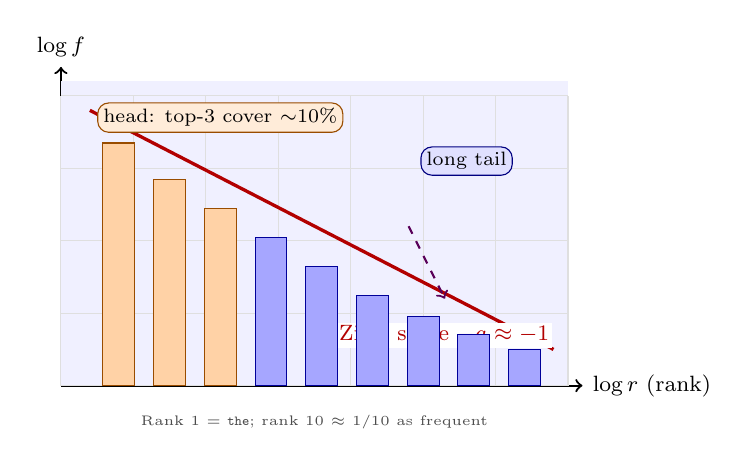
\begin{tikzpicture}[scale=0.92, font=\footnotesize]
  % axes
  \draw[->, thick] (0,0) -- (7.2,0) node[right] {$\log r$ (rank)};
  \draw[->, thick] (0,0) -- (0,4.4) node[above] {$\log f$};
  \fill[blue!6] (0,0) rectangle (7,4.2);
  \draw[gray!25] (0,0) grid (7,4.0);
  % ideal Zipf line
  \draw[very thick, red!70!black] (0.4,3.8) -- (6.8,0.5) node[above left, fill=white, inner sep=1pt] {Zipf: slope $-a\approx-1$};
  % bars for actual frequencies (simulated)
  \foreach \x/\h in {0.8/3.35, 1.5/2.85, 2.2/2.45, 2.9/2.05, 3.6/1.65, 4.3/1.25, 5.0/0.95, 5.7/0.70, 6.4/0.50} {
    \fill[blue!35, draw=blue!60!black] (\x-0.22,0) rectangle (\x+0.22,\h);
  }
  \foreach \x/\h in {0.8/3.35, 1.5/2.85, 2.2/2.45} {
    \fill[orange!35, draw=orange!60!black] (\x-0.22,0) rectangle (\x+0.22,\h);
  }
  \node[fill=orange!15, draw=orange!60!black, rounded corners, inner sep=2pt, font=\scriptsize] at (2.2,3.7) {head: top-3 cover $\sim$10\%};
  \node[fill=blue!12, draw=blue!50!black, rounded corners, inner sep=2pt, font=\scriptsize] at (5.6,3.1) {long tail};
  \draw[->, violet!70!black, thick, dashed] (4.8,2.2) -- (5.3,1.2);
  \node[font=\tiny, text=gray!60!black] at (3.5,-0.5) {Rank 1 = \texttt{the}; rank 10 $\approx$ 1/10 as frequent};
\end{tikzpicture}
\end{center}

Why care? The tail tells us smoothing and subwords are not optional -- any model that assigns zero probability to unseen $n$-grams will fail on real text.

\section{$n$-Grams: Predicting the Next Token}
If we know the previous words, can we guess the next? An $n$-gram model says yes, using only the last $n-1$ tokens.

\begin{definition}[$n$-Gram and Markov Assumption]
Let $w_1^m = w_1,\dots,w_m$ be a token sequence. An \textbf{$n$-gram} is a contiguous subsequence of length $n$. The model makes a $(n-1)$-th order Markov assumption:
\begin{equation}
P(w_1^m) \;=\; \prod_{i=1}^{m} P(w_i\mid w_1^{i-1}) \;\approx\; \prod_{i=1}^{m} P(w_i\mid w_{i-n+1}^{i-1}),
\end{equation}
with $w_j = \langle s\rangle$ (start) for $j\le 0$ and $w_{m+1}=\langle /s\rangle$ for sentence end. When $n=1,2,3$ we call them unigram, bigram, trigram.
\end{definition}

\begin{center}
\begin{tikzpicture}[font=\footnotesize, >=Stealth]
  \foreach \i/\w in {1/the,2/cat,3/sat,4/on,5/the,6/mat} {
    \node[draw, fill=green!15, rounded corners, minimum width=1.1cm, minimum height=0.75cm] (t\i) at (1.45*\i,1.2) {\w};
  }
  \node[font=\scriptsize, text=gray!60!black] at (5.2,2.1) {tokens $w_1\dots w_6$};
  \node[draw, fill=blue!15, thick, rounded corners, fit=(t1)(t2), inner sep=3pt, label={[font=\scriptsize, text=blue!60!black]below:bigram 1}] (b1) {};
  \node[draw, fill=orange!15, thick, rounded corners, fit=(t2)(t3), inner sep=3pt, label={[font=\scriptsize, text=orange!60!black]below:bigram 2}] (b2) {};
  \node[draw, fill=violet!12, thick, rounded corners, fit=(t3)(t4), inner sep=3pt, label={[font=\scriptsize, text=violet!60!black]below:bigram 3}] (b3) {};
  \node at (8.8,1.2) {\dots};
  \draw[->, thick, red!70!black] (5.2,0.05) -- (5.2,-0.55) node[below, align=center, font=\scriptsize, fill=red!8, draw=red!40!black, rounded corners, inner sep=2pt] {slide window\\$n=2$: $P(\text{sat}\mid\text{cat})$\\$n=3$: $P(\text{sat}\mid\text{the cat})$};
  \node[font=\scriptsize, text=gray!60!black] at (5.2,-1.7) {MLE counts from corpus};
\end{tikzpicture}
\end{center}

Maximum likelihood estimation is just counting.

\begin{definition}[MLE for $n$-Grams]
Let $c(\cdot)$ be corpus counts. Then
\begin{equation}
P_{\text{MLE}}(w_i\mid w_{i-n+1}^{i-1}) \;=\; \frac{c(w_{i-n+1}^{i})}{c(w_{i-n+1}^{i-1})}.
\end{equation}
In particular, for bigrams
\begin{equation}
P(w_i\mid w_{i-1})=\frac{c(w_{i-1},w_i)}{c(w_{i-1})},
\end{equation}
and for trigrams
\begin{equation}
P(w_i\mid w_{i-2},w_{i-1})=\frac{c(w_{i-2},w_{i-1},w_i)}{c(w_{i-2},w_{i-1})}.
\end{equation}
\end{definition}

\begin{example}[Tiny Corpus]
Corpus: \texttt{<s> the cat sat} and \texttt{<s> the cat ran}. Then $c(\text{the})=2$, $c(\text{the cat})=2$, $c(\text{cat sat})=1$. So $P(\text{cat}\mid\text{the})=2/2=1.0$, $P(\text{sat}\mid\text{cat})=1/2=0.5$. Any unseen bigram like $(\text{ran},\text{the})$ gets probability $0$ -- the sparsity problem that motivates smoothing (Chapter~5).
\end{example}

\begin{lstlisting}[language=Python]
from collections import Counter, defaultdict

corpus = ["<s> the cat sat </s>", "<s> the cat ran </s>"]
# bigram MLE
bigram_counts = Counter()
unigram_counts = Counter()
for sent in corpus:
    toks = sent.split()
    for i, w in enumerate(toks):
        unigram_counts[w] += 1
        if i > 0:
            bigram_counts[(toks[i-1], w)] += 1

def p_mle(prev, word):
    return bigram_counts[(prev, word)] / unigram_counts[prev] if unigram_counts[prev] else 0.0

print("P(cat|the) =", p_mle("the", "cat"))   # 1.0
print("P(sat|cat) =", p_mle("cat", "sat"))   # 0.5
print("P(mat|cat) =", p_mle("cat", "mat"))   # 0.0 -> need smoothing
\end{lstlisting}

\subsection*{Chapter Summary}
Text $\to$ normalization $\to$ tokenization $\to$ integer IDs. Token vs.\ type vs.\ vocabulary; word vocabularies are large and leaky, so BPE merges frequent pairs into subwords. Word frequencies follow Zipf $f\propto 1/r^{a}$ (straight on log--log), implying a heavy tail. $n$-grams model $P(w_i\mid n-1\text{ history})$ by MLE ratios of counts; sparsity forces smoothing next chapter.

\section{Exercises}
\begin{exercise} Token/type/vocabulary. Sentence: ``Buffalo buffalo Buffalo buffalo.'' After lowercasing and stripping punctuation you get [\texttt{buffalo, buffalo, buffalo, buffalo}]. How many tokens? How many types? Give $|\mathcal{V}|$. If a tokenizer keeps case, how do answers change? \end{exercise}
\begin{exercise} BPE trace. Corpus words: \texttt{["ab","ac","ab","ad"]} with characters plus \texttt{</w>}. Show the first two BPE merges and the resulting tokenizations. Why does BPE prefer \texttt{ab} as a merged type over \texttt{ac}? \end{exercise}
\begin{exercise} Zipf calculation. Suppose $a=1$, $C$ chosen so $\sum_{r=1}^{V} C/r =1$ with $V=10\,000$. Estimate $C$ (harmonic number $H_{10000}\approx 9.21$) and compute $f(1), f(10), f(100)$. What fraction of probability mass is in the top-10 ranks? \end{exercise}
\begin{exercise} Bigram MLE by hand. Corpus: three sentences \texttt{<s> a b a}, \texttt{<s> a b}, \texttt{<s> b a}. Compute $c(a)$, $c(b)$, $c(a,b)$, $c(b,a)$, $c(\langle s\rangle,a)$ and then $P(b\mid a)$, $P(a\mid b)$, $P(a\mid \langle s\rangle)$. Verify each history sums to $1$. \end{exercise}
\begin{exercise} Sparsity and smoothing intuition. Your bigram model trained above assigns $P(\text{mat}\mid\text{cat})=0$. Explain why this zeroes the probability of any sentence containing \texttt{cat mat}, and propose two fixes (add-one smoothing and subword splitting) with one pro and one con each. \end{exercise}

